\documentclass{article}
\usepackage[dvips]{graphicx}
\usepackage{fancyhdr,url}
\usepackage[utf8]{inputenc}
\usepackage[pdftitle={skymap}, pdfauthor={Arthur Rosso}, pdfsubject={Crie seu próprio skymap}, pdfkeywords={Crie seu próprio skymap}, colorlinks=true, linkcolor=blue, citecolor=blue, filecolor=blue, urlcolor=blue]{hyperref}
\usepackage[T1]{fontenc}
\usepackage{xcolor}
\usepackage[a4paper, portrait, left=0.6cm, right=1.5cm, top=0.4cm, bottom=0.45in]{geometry}
\usepackage{array}
\pagecolor{black}
\color{white}

\title{Faça seu próprio planisfério}
\author{Arthur Rosso}
\date{2019}

\begin{document}
\thispagestyle{empty}

\setlength{\arrayrulewidth}{3mm}
\begin{center}
{
\begin{tabular}{ |c|c|c|  }
\hline
\\ 
\\ 
\\ 
\multicolumn{3}{|c|}{
    \begin{LARGE}
    \centerline{I love you to the moon and back.}
    \end{LARGE}
} 
\\ 
\\ 
\multicolumn{3}{|c|}{
    \centerline{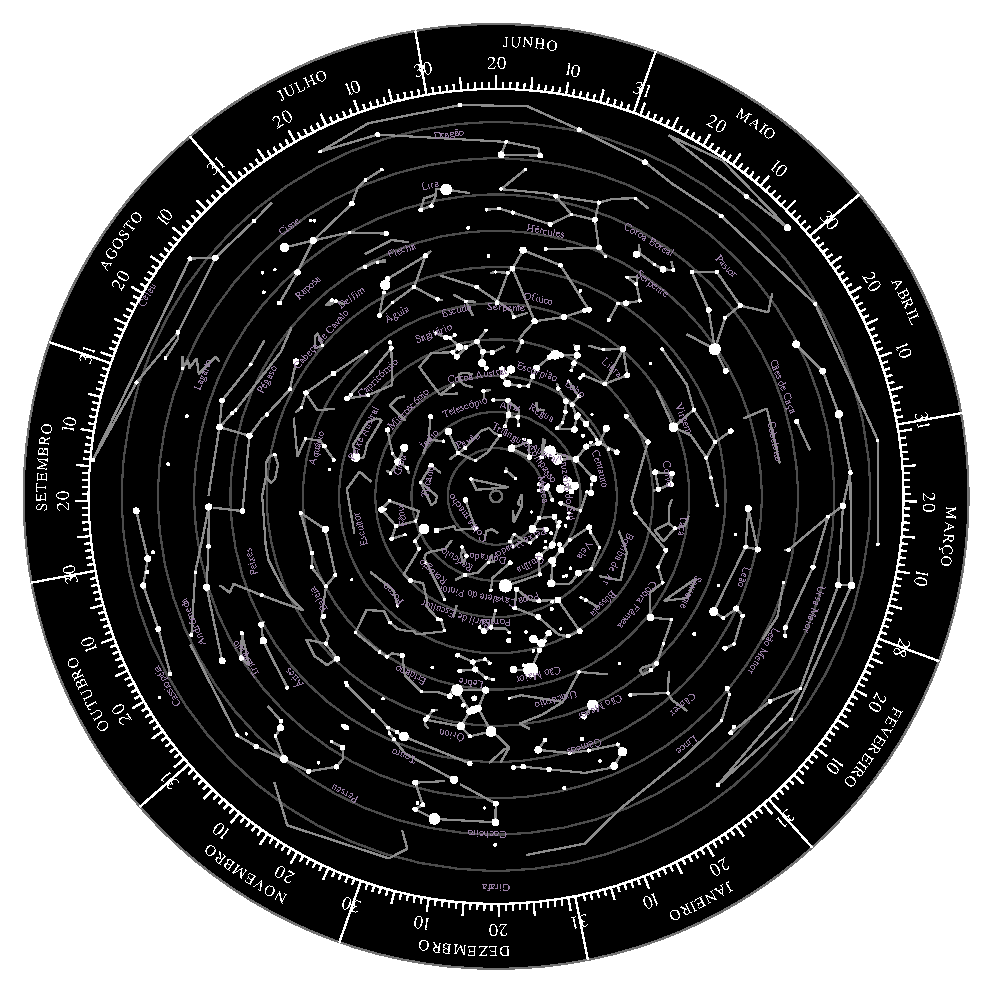
\includegraphics{tmp/starwheel}}
} 
\\
\\
\\
\\
\\
\\
\\
\\
\\
\\
\\
\\
\\ \hspace{19.27cm}
\\
\multicolumn{3}{|c|}{
    \begin{LARGE}
    \centerline{The night we match ;) .}
    \end{LARGE}
}
\\
\\
\multicolumn{3}{|c|}{
    \begin{large}
    \centerline{Stars above Canoas, RS, BR on the 1st January, 2019, at 12:00 am.}
    \end{large}
} 
\\
\\
\\
\hline
\end{tabular}
}
\end{center}

\end{document}